\documentclass[12pt,a4paper]{article}

% Packages
\usepackage{amsmath}
\usepackage{amssymb}
\usepackage{amsthm}
\usepackage[margin=1in]{geometry}
\usepackage{enumitem}
\usepackage{xcolor}
\usepackage{mathtools}
\usepackage{tikz}

% Custom environments
\newtheorem{explanation}{Explanation}
\theoremstyle{definition}
\newtheorem{solution}{Solution}

% Custom commands
\newcommand{\stage}[1]{\textbf{\textcolor{blue}{#1}}}

% Title information
\title{Methods of Applied Mathematics - Part 1\\
Exercise Sheet 2: Question 2\\
Multiple Equilibria in a 1-Dimensional System}
\author{Complete Solution with XYZ Methodology}
\date{}

\begin{document}

\maketitle

\section*{Problem Statement}

Consider the dynamical system:
\begin{equation}
\dot{x} = x^4 - 17x^3 + 101x^2 - 247x + 210
\end{equation}

You are told that this has four equilibria, at $x = 2, 3, 5, 7$.

\section{Question 2(a): Factorized Form of the ODE}

\begin{solution}

\subsection*{Step 1: Understand the Relationship Between Roots and Factorization}

\begin{itemize}[leftmargin=*]
\item \stage{STAGE X (What we know):} We have a polynomial $p(x) = x^4 - 17x^3 + 101x^2 - 247x + 210$, and we're told it has roots at $x = 2, 3, 5, 7$. These are the equilibria where $\dot{x} = 0$.

\item \stage{STAGE Y (Why factorization works):} By the \textbf{Fundamental Theorem of Algebra}, a degree-4 polynomial with roots $r_1, r_2, r_3, r_4$ can be written as:
\begin{equation}
p(x) = A(x - r_1)(x - r_2)(x - r_3)(x - r_4)
\end{equation}
where $A$ is the leading coefficient. Since our polynomial has leading coefficient 1 (the $x^4$ term), we have $A = 1$.

\item \stage{STAGE Z (What we'll show):} We'll verify that $(x-2)(x-3)(x-5)(x-7)$ equals the given polynomial, thus identifying $a = 2, b = 3, c = 5, d = 7$.
\end{itemize}

\subsection*{Step 2: Write the Factorized Form}

Since the equilibria are at $x = 2, 3, 5, 7$, the factorized form must be:
\begin{equation}
\dot{x} = (x - 2)(x - 3)(x - 5)(x - 7)
\end{equation}

Therefore:
\begin{equation}
\boxed{a = 2, \quad b = 3, \quad c = 5, \quad d = 7}
\end{equation}

\subsection*{Step 3: Verify by Expansion (ESSENTIAL)}

We must verify that $(x-2)(x-3)(x-5)(x-7)$ expands to $x^4 - 17x^3 + 101x^2 - 247x + 210$.

\textbf{Step 3A: Expand in Pairs}

First pair:
\begin{align}
(x - 2)(x - 3) &= x^2 - 3x - 2x + 6 \\
&= x^2 - 5x + 6
\end{align}

Second pair:
\begin{align}
(x - 5)(x - 7) &= x^2 - 7x - 5x + 35 \\
&= x^2 - 12x + 35
\end{align}

\textbf{Step 3B: Multiply the Results}

\begin{align}
(x^2 - 5x + 6)(x^2 - 12x + 35) &= x^2(x^2 - 12x + 35) - 5x(x^2 - 12x + 35) + 6(x^2 - 12x + 35) \\
&= x^4 - 12x^3 + 35x^2 \\
&\quad - 5x^3 + 60x^2 - 175x \\
&\quad + 6x^2 - 72x + 210
\end{align}

Collecting like terms:
\begin{align}
&= x^4 + (-12 - 5)x^3 + (35 + 60 + 6)x^2 + (-175 - 72)x + 210 \\
&= x^4 - 17x^3 + 101x^2 - 247x + 210 \quad \checkmark
\end{align}

\begin{explanation}[Verification Confirms Factorization]
The expansion matches the original polynomial exactly. This confirms that:
\begin{equation}
x^4 - 17x^3 + 101x^2 - 247x + 210 = (x-2)(x-3)(x-5)(x-7)
\end{equation}
\end{explanation}

\subsection*{Step 4: Alternative Verification Using Vieta's Formulas}

For completeness, we can verify using Vieta's formulas. For a monic polynomial $x^4 + px^3 + qx^2 + rx + s$ with roots $\alpha, \beta, \gamma, \delta$:

\begin{align}
\alpha + \beta + \gamma + \delta &= -p \\
\alpha\beta + \alpha\gamma + \alpha\delta + \beta\gamma + \beta\delta + \gamma\delta &= q \\
\alpha\beta\gamma + \alpha\beta\delta + \alpha\gamma\delta + \beta\gamma\delta &= -r \\
\alpha\beta\gamma\delta &= s
\end{align}

With roots $2, 3, 5, 7$:

\begin{align}
\text{Sum: } & 2 + 3 + 5 + 7 = 17 = -(-17) \quad \checkmark \\
\text{Pairwise products: } & 2 \cdot 3 + 2 \cdot 5 + 2 \cdot 7 + 3 \cdot 5 + 3 \cdot 7 + 5 \cdot 7 \\
& = 6 + 10 + 14 + 15 + 21 + 35 = 101 \quad \checkmark \\
\text{Triple products: } & 2 \cdot 3 \cdot 5 + 2 \cdot 3 \cdot 7 + 2 \cdot 5 \cdot 7 + 3 \cdot 5 \cdot 7 \\
& = 30 + 42 + 70 + 105 = 247 = -(-247) \quad \checkmark \\
\text{Product of all: } & 2 \cdot 3 \cdot 5 \cdot 7 = 210 \quad \checkmark
\end{align}

All checks pass!

\subsection*{Final Answer for Part (a)}

\begin{equation}
\boxed{
\begin{aligned}
\dot{x} &= (x - a)(x - b)(x - c)(x - d) \\
\text{where } & a = 2, \quad b = 3, \quad c = 5, \quad d = 7
\end{aligned}
}
\end{equation}

\end{solution}

\vspace{10pt}
\hrule
\vspace{10pt}

\section{Question 2(b): Stability of Each Equilibrium}

\begin{solution}

\subsection*{Step 1: Method Selection for Stability Analysis}

\begin{itemize}[leftmargin=*]
\item \stage{STAGE X (What we need):} Determine whether each equilibrium at $x^* = 2, 3, 5, 7$ is stable or unstable.

\item \stage{STAGE Y (Why linearization):} From Lecture Notes (Section 9, page 32), for a 1D system $\dot{x} = f(x)$ with equilibrium at $x^*$:
\begin{equation}
\text{Stability coefficient: } \lambda = \frac{df}{dx}\bigg|_{x=x^*} = f'(x^*)
\end{equation}
\begin{itemize}
\item If $\lambda < 0$: equilibrium is \textbf{stable} (attractor)
\item If $\lambda > 0$: equilibrium is \textbf{unstable} (repeller)
\end{itemize}

\item \stage{STAGE Z (Our approach):} Calculate $f'(x)$ in factored form (easier than expanding), then evaluate at each equilibrium point.
\end{itemize}

\subsection*{Step 2: Compute the Derivative Using Product Rule}

Given $f(x) = (x-2)(x-3)(x-5)(x-7)$, we need $f'(x)$.

\textbf{Product Rule for Four Factors:}

For $f(x) = u_1 \cdot u_2 \cdot u_3 \cdot u_4$ where $u_i = (x - a_i)$:
\begin{equation}
f'(x) = u_1' u_2 u_3 u_4 + u_1 u_2' u_3 u_4 + u_1 u_2 u_3' u_4 + u_1 u_2 u_3 u_4'
\end{equation}

Since $u_i' = 1$ for all factors:
\begin{equation}
f'(x) = (x-3)(x-5)(x-7) + (x-2)(x-5)(x-7) + (x-2)(x-3)(x-7) + (x-2)(x-3)(x-5)
\end{equation}

\begin{explanation}[Key Observation for Evaluation]
At an equilibrium $x^* = a_i$, one factor $(x - a_i)$ equals zero. When computing $f'(x^*)$, all terms containing $(x^* - a_i)$ vanish, leaving only the term where that factor was differentiated.

For example, at $x^* = 2$:
\begin{align}
f'(2) &= \underbrace{(2-3)(2-5)(2-7)}_{(x-2)' \text{ term, survives}} + \underbrace{(2-2)(\ldots)}_{=0} + \underbrace{(2-2)(\ldots)}_{=0} + \underbrace{(2-2)(\ldots)}_{=0} \\
&= (-1)(-3)(-5) = -15
\end{align}
\end{explanation}

\subsection*{Step 3: Evaluate $f'(x)$ at Each Equilibrium}

\textbf{At $x^* = 2$:}
\begin{align}
f'(2) &= (2-3)(2-5)(2-7) \\
&= (-1)(-3)(-5) \\
&= -15 < 0 \quad \Rightarrow \quad \boxed{\text{STABLE}}
\end{align}

\textbf{At $x^* = 3$:}
\begin{align}
f'(3) &= (3-2)(3-5)(3-7) \\
&= (1)(-2)(-4) \\
&= 8 > 0 \quad \Rightarrow \quad \boxed{\text{UNSTABLE}}
\end{align}

\textbf{At $x^* = 5$:}
\begin{align}
f'(5) &= (5-2)(5-3)(5-7) \\
&= (3)(2)(-2) \\
&= -12 < 0 \quad \Rightarrow \quad \boxed{\text{STABLE}}
\end{align}

\textbf{At $x^* = 7$:}
\begin{align}
f'(7) &= (7-2)(7-3)(7-5) \\
&= (5)(4)(2) \\
&= 40 > 0 \quad \Rightarrow \quad \boxed{\text{UNSTABLE}}
\end{align}

\subsection*{Step 4: Physical Interpretation via Phase Line}

To understand the dynamics, construct the phase line showing $\dot{x}$ in each region:

\begin{center}
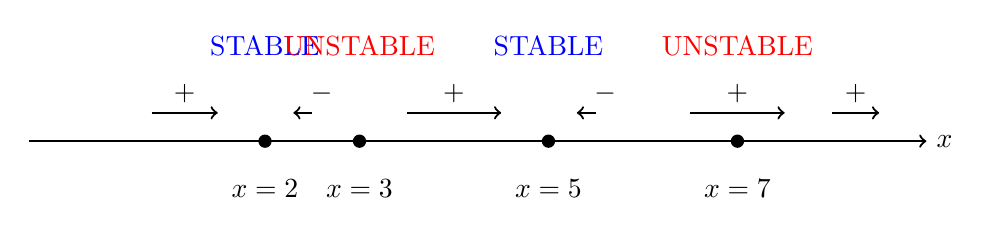
\begin{tikzpicture}[scale=1.2]
% Axis
\draw[thick,->] (-0.5,0) -- (9,0) node[right] {$x$};

% Equilibrium points
\foreach \x/\label in {2/2, 3/3, 5/5, 7/7} {
    \fill (\x,0) circle (2pt);
    \node[below] at (\x,-0.3) {$x=\x$};
}

% Stability labels
\node[above, blue] at (2,0.8) {STABLE};
\node[above, red] at (3,0.8) {UNSTABLE};
\node[above, blue] at (5,0.8) {STABLE};
\node[above, red] at (7,0.8) {UNSTABLE};

% Arrows showing direction
\draw[->, thick] (0.8,0.3) -- (1.5,0.3);
\node[above] at (1.15,0.3) {$+$};

\draw[->, thick] (2.5,0.3) -- (2.3,0.3);
\node[above] at (2.6,0.3) {$-$};

\draw[->, thick] (3.5,0.3) -- (4.5,0.3);
\node[above] at (4,0.3) {$+$};

\draw[->, thick] (5.5,0.3) -- (5.3,0.3);
\node[above] at (5.6,0.3) {$-$};

\draw[->, thick] (6.5,0.3) -- (7.5,0.3);
\node[above] at (7,0.3) {$+$};

\draw[->, thick] (8,0.3) -- (8.5,0.3);
\node[above] at (8.25,0.3) {$+$};
\end{tikzpicture}
\end{center}

\begin{explanation}[Understanding the Phase Line]
\textbf{Sign Analysis:}

In each region, determine the sign of $\dot{x} = (x-2)(x-3)(x-5)(x-7)$:

\begin{itemize}
\item $x < 2$: All four factors negative $\Rightarrow (-)(-)(-)(-) = (+) \Rightarrow \dot{x} > 0$ (moving right)
\item $2 < x < 3$: Three factors negative, one positive $\Rightarrow (+)(-)(-)(-) = (-) \Rightarrow \dot{x} < 0$ (moving left toward 2)
\item $3 < x < 5$: Two factors negative, two positive $\Rightarrow (+)(+)(-)(-)= (+) \Rightarrow \dot{x} > 0$ (moving right)
\item $5 < x < 7$: One factor negative, three positive $\Rightarrow (+)(+)(+)(-) = (-) \Rightarrow \dot{x} < 0$ (moving left toward 5)
\item $x > 7$: All factors positive $\Rightarrow (+)(+)(+)(+) = (+) \Rightarrow \dot{x} > 0$ (moving right to $\infty$)
\end{itemize}

\textbf{Stability Pattern:}
\begin{itemize}
\item At $x = 2$: Arrows point toward it from both sides $\Rightarrow$ STABLE
\item At $x = 3$: Arrows point away from it on both sides $\Rightarrow$ UNSTABLE
\item At $x = 5$: Arrows point toward it from both sides $\Rightarrow$ STABLE
\item At $x = 7$: Arrows point away from it on both sides $\Rightarrow$ UNSTABLE
\end{itemize}

This confirms our linearization analysis!
\end{explanation}

\subsection*{Step 5: Pattern Recognition}

\begin{explanation}[General Pattern for Multiple Equilibria]
Notice the alternating stability pattern: STABLE - UNSTABLE - STABLE - UNSTABLE.

\textbf{Why this happens:}
\begin{itemize}
\item Between two adjacent equilibria, $\dot{x}$ must have constant sign (continuous function, no zeros in between)
\item At each equilibrium, the function crosses zero (changes sign)
\item Starting from $x \to -\infty$: For large negative $x$, the leading term is $x^4 > 0$, so eventually $\dot{x} > 0$
\item Each zero crossing alternates the sign of $\dot{x}$
\item Stability alternates: if arrows approach from the left and leave to the right (stable), the next equilibrium must have arrows approach from left and right (unstable), and so on
\end{itemize}

\textbf{General Rule (Lecture Notes, Section 6):} In 1D systems, adjacent equilibria must have opposite stability.
\end{explanation}

\subsection*{Final Answer for Part (b)}

\begin{equation}
\boxed{
\begin{array}{|c|c|c|c|}
\hline
\text{Equilibrium } x^* & f'(x^*) & \text{Sign} & \text{Stability} \\
\hline
2 & -15 & - & \text{STABLE (attractor)} \\
3 & +8 & + & \text{UNSTABLE (repeller)} \\
5 & -12 & - & \text{STABLE (attractor)} \\
7 & +40 & + & \text{UNSTABLE (repeller)} \\
\hline
\end{array}
}
\end{equation}

\end{solution}

\vspace{10pt}
\hrule
\vspace{10pt}

\section{Question 2(c): Long-Term Behavior from $x_0 = 6$}

\begin{solution}

\subsection*{Step 1: Identify Initial Position on Phase Line}

\begin{itemize}[leftmargin=*]
\item \stage{STAGE X (What we know):} The initial condition is $x_0 = 6$, which lies between the equilibria at $x = 5$ and $x = 7$.

\item \stage{STAGE Y (Why location matters):} From the phase line analysis in part (b), we determined the sign of $\dot{x}$ in the interval $(5, 7)$. This tells us which direction the trajectory moves.

\item \stage{STAGE Z (What we'll determine):} We'll find which equilibrium the trajectory approaches as $t \to \infty$.
\end{itemize}

\subsection*{Step 2: Determine Sign of $\dot{x}$ at $x_0 = 6$}

From part (b), in the region $5 < x < 7$:
\begin{align}
\dot{x} &= (x-2)(x-3)(x-5)(x-7) \\
&= (+)(+)(+)(-) \\
&= (-) < 0
\end{align}

At $x = 6$ specifically:
\begin{align}
\dot{x}\big|_{x=6} &= (6-2)(6-3)(6-5)(6-7) \\
&= (4)(3)(1)(-1) \\
&= -12 < 0 \quad \checkmark
\end{align}

\subsection*{Step 3: Determine Direction of Motion}

Since $\dot{x} < 0$ at $x_0 = 6$:
\begin{equation}
\frac{dx}{dt} < 0 \quad \Rightarrow \quad x \text{ is \textbf{decreasing}}
\end{equation}

The trajectory moves to the \textbf{left} (toward smaller values of $x$).

\subsection*{Step 4: Identify the Attractor}

Starting at $x_0 = 6$ and moving left:
\begin{itemize}
\item The trajectory is in the region $(5, 7)$ where $\dot{x} < 0$ throughout
\item Moving left, the trajectory approaches $x = 5$
\item From part (b), $x = 5$ is a STABLE equilibrium (attractor)
\item The trajectory cannot cross the equilibrium (by uniqueness of solutions)
\end{itemize}

\begin{explanation}[Why $x = 5$ is the Long-Term Destination]
\textbf{Basin of Attraction:}

The basin of attraction of $x = 5$ consists of all initial conditions that eventually approach $x = 5$.

From the phase line:
\begin{itemize}
\item For $x \in (3, 5)$: $\dot{x} > 0$, trajectories move right toward $x = 5$
\item For $x \in (5, 7)$: $\dot{x} < 0$, trajectories move left toward $x = 5$
\end{itemize}

Therefore, the basin of attraction is the entire interval $(3, 7)$.

Since $x_0 = 6 \in (3, 7)$, the trajectory must approach $x = 5$.
\end{explanation}

\subsection*{Step 5: Characterize the Approach}

Near the stable equilibrium $x = 5$, the linearization gives:
\begin{equation}
\dot{x} \approx f'(5) \cdot (x - 5) = -12(x - 5)
\end{equation}

This has solution:
\begin{equation}
x(t) - 5 \approx (x_0 - 5)e^{-12t} = (6 - 5)e^{-12t} = e^{-12t}
\end{equation}

Therefore:
\begin{equation}
x(t) \approx 5 + e^{-12t}
\end{equation}

The approach is \textbf{exponential decay} with rate constant $\lambda = 12$, giving a time scale $\tau = 1/12 \approx 0.083$.

\subsection*{Final Answer for Part (c)}

\begin{equation}
\boxed{
\begin{aligned}
&\text{Starting from } x_0 = 6: \\
&\text{Long-term behavior: } x(t) \to 5 \text{ as } t \to \infty \\
&\text{Approach: Exponential decay with rate } \lambda = 12 \\
&\text{Time scale: } \tau = 1/12 \approx 0.083
\end{aligned}
}
\end{equation}

\textbf{Physical Description:} The trajectory decreases monotonically from $x_0 = 6$ toward the stable equilibrium at $x = 5$, approaching it exponentially with approximately 95\% of convergence achieved by $t \approx 0.25$.

\end{solution}

\vspace{10pt}
\hrule
\vspace{10pt}

\section{Question 2(d): Long-Term Behavior from $x_0 = 8$}

\begin{solution}

\subsection*{Step 1: Identify Initial Position on Phase Line}

\begin{itemize}[leftmargin=*]
\item \stage{STAGE X (What we know):} The initial condition is $x_0 = 8$, which lies beyond all equilibria: $8 > 7 > 5 > 3 > 2$.

\item \stage{STAGE Y (Why this is different):} Unlike part (c), we're not between two equilibria. We're in the unbounded region $x > 7$. This means the trajectory might escape to infinity.

\item \stage{STAGE Z (What we'll determine):} Whether the trajectory approaches an equilibrium or diverges to $+\infty$.
\end{itemize}

\subsection*{Step 2: Determine Sign of $\dot{x}$ for $x > 7$}

From part (b), in the region $x > 7$:
\begin{align}
\dot{x} &= (x-2)(x-3)(x-5)(x-7) \\
&= (+)(+)(+)(+) \\
&= (+) > 0
\end{align}

At $x = 8$ specifically:
\begin{align}
\dot{x}\big|_{x=8} &= (8-2)(8-3)(8-5)(8-7) \\
&= (6)(5)(3)(1) \\
&= 90 > 0 \quad \checkmark
\end{align}

\subsection*{Step 3: Determine Direction of Motion}

Since $\dot{x} > 0$ at $x_0 = 8$:
\begin{equation}
\frac{dx}{dt} > 0 \quad \Rightarrow \quad x \text{ is \textbf{increasing}}
\end{equation}

The trajectory moves to the \textbf{right} (toward larger values of $x$).

\subsection*{Step 4: Analyze Long-Term Behavior}

\textbf{Key Observation:}
\begin{itemize}
\item For all $x > 7$: $\dot{x} > 0$ (from phase line analysis)
\item As $x$ increases, $\dot{x}$ also increases (positive feedback)
\item There are no equilibria to the right of $x = 7$ to stop the growth
\end{itemize}

\begin{explanation}[Why Trajectory Escapes to Infinity]
\textbf{Asymptotic Analysis:}

For large $x$, the polynomial behaves like its leading term:
\begin{equation}
\dot{x} = x^4 - 17x^3 + 101x^2 - 247x + 210 \sim x^4 \text{ as } x \to \infty
\end{equation}

This gives:
\begin{equation}
\frac{dx}{dt} \sim x^4 \quad \text{for large } x
\end{equation}

Separating variables:
\begin{align}
\frac{dx}{x^4} &\sim dt \\
\int_{x_0}^{x(t)} \frac{ds}{s^4} &\sim \int_0^t d\tau \\
-\frac{1}{3x^3}\bigg|_{x_0}^{x(t)} &\sim t \\
-\frac{1}{3x(t)^3} + \frac{1}{3x_0^3} &\sim t
\end{align}

Solving for $x(t)$:
\begin{equation}
\frac{1}{x(t)^3} \sim \frac{1}{x_0^3} - 3t
\end{equation}

This blows up (becomes singular) when:
\begin{equation}
t_{\text{blow-up}} \sim \frac{1}{3x_0^3} = \frac{1}{3 \cdot 8^3} = \frac{1}{1536} \approx 0.00065
\end{equation}

The trajectory reaches infinity in \textbf{finite time}!
\end{explanation}

\subsection*{Step 5: Verify with Qualitative Reasoning}

\begin{explanation}[Finite-Time Blow-Up Mechanism]
From Lecture Notes (Section 6): For $\dot{x} = f(x)$, if $f(x) \to \infty$ faster than linearly as $x \to \infty$, trajectories can escape to infinity in finite time.

\textbf{Intuition:}
\begin{itemize}
\item At $x = 8$: $\dot{x} = 90$ (already quite large)
\item As $x$ grows, $\dot{x} \sim x^4$ grows even faster
\item The rate of growth accelerates without bound
\item The accumulated distance $\int \dot{x} \, dt$ diverges in finite time
\end{itemize}

\textbf{Contrast with Exponential Growth:}
\begin{itemize}
\item If $\dot{x} = x$: solution is $x(t) = x_0 e^t$, which reaches infinity only as $t \to \infty$
\item Here $\dot{x} = x^4$: superlinear growth causes finite-time blow-up
\end{itemize}
\end{explanation}

\subsection*{Step 6: Exact Blow-Up Time Estimate}

For $x_0 = 8$, the asymptotic estimate gives:
\begin{equation}
t_{\text{blow-up}} \approx \frac{1}{3 \cdot 8^3} = \frac{1}{1536} \approx 6.5 \times 10^{-4}
\end{equation}

This is an approximation valid for large $x$. The actual blow-up time might differ slightly, but the order of magnitude is correct.

\subsection*{Final Answer for Part (d)}

\begin{equation}
\boxed{
\begin{aligned}
&\text{Starting from } x_0 = 8: \\
&\text{Long-term behavior: } x(t) \to +\infty \text{ as } t \to t_{\text{blow-up}} \\
&\text{Type: \textbf{Finite-time blow-up}} \\
&\text{Blow-up time: } t_{\text{blow-up}} \approx \frac{1}{3x_0^3} = \frac{1}{1536} \approx 6.5 \times 10^{-4} \\
&\text{Mechanism: Superlinear growth } (\dot{x} \sim x^4 \text{ for large } x)
\end{aligned}
}
\end{equation}

\textbf{Physical Description:} The trajectory increases monotonically from $x_0 = 8$, accelerating rapidly as $\dot{x} \sim x^4$. The solution becomes unbounded (reaches infinity) in finite time, approximately $t \approx 0.00065$. This is a characteristic behavior of superlinearly growing systems.

\end{solution}

\vspace{10pt}
\hrule
\vspace{10pt}

\section*{Summary: Global Phase Portrait of the System}

\subsection*{Complete Classification of Long-Term Behaviors}

For the system $\dot{x} = (x-2)(x-3)(x-5)(x-7)$:

\begin{enumerate}[leftmargin=*]
\item \textbf{Basin of $x = 2$}: Initial conditions $x_0 \in (-\infty, 3)$ $\Rightarrow$ $x(t) \to 2$ as $t \to \infty$

\item \textbf{Basin of $x = 5$}: Initial conditions $x_0 \in (3, 7)$ $\Rightarrow$ $x(t) \to 5$ as $t \to \infty$

\item \textbf{Escape to $+\infty$}: Initial conditions $x_0 \in (7, \infty)$ $\Rightarrow$ $x(t) \to +\infty$ in finite time

\item \textbf{Unstable equilibria}: $x = 3$ and $x = 7$ are repellers (no basin of attraction)
\end{enumerate}

\subsection*{Key Insights from Lecture Notes}

\begin{itemize}[leftmargin=*]
\item \textbf{Alternating stability}: Adjacent equilibria have opposite stability (Section 6)

\item \textbf{Basins separated by unstable equilibria}: The unstable points at $x = 3$ and $x = 7$ form boundaries between different basins of attraction

\item \textbf{Finite-time blow-up}: Possible when $\dot{x}$ grows superlinearly (faster than linear) as $|x| \to \infty$

\item \textbf{Phase line is the complete picture}: In 1D, the phase line fully determines all long-term behaviors (no hidden complexity like limit cycles, which are impossible in 1D)
\end{itemize}

\end{document}
